%!TEX root = ../paper.tex

% Small differences in anisotropy  
	In \cref{s:results} some small differences between the anisotropies of the different kernels were observed. This section attempts to find an explanation for this effect.

	% Single Sphere
			\begin{figure}
				\centering
				\begin{subfigure}{0.23\textwidth}
					\centering
					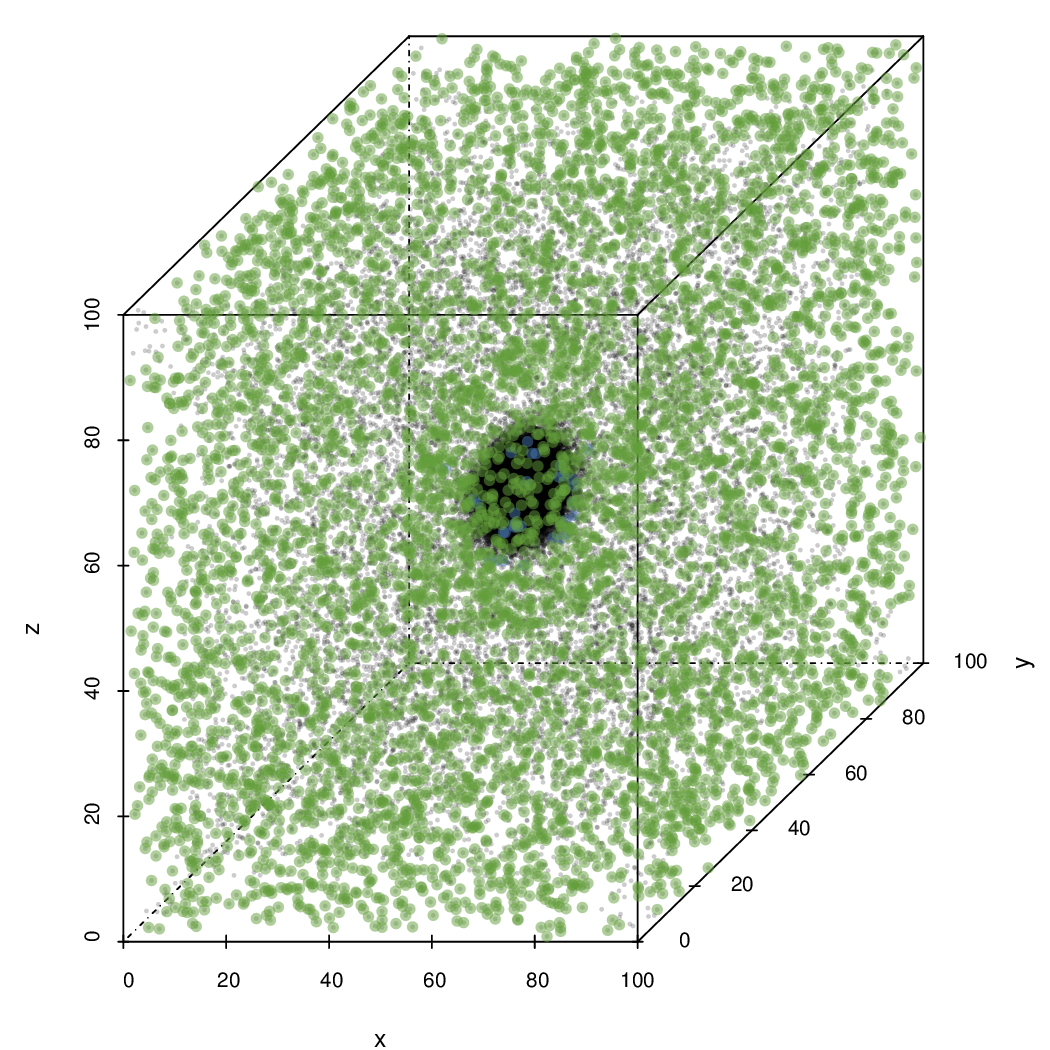
\includegraphics[keepaspectratio=true, width=\textwidth, height=0.23\textheight]{discussion/img/ferdosi_1_60000_anisotropy.png}
					\caption{\ferdosiOne [\num{2.783732800937043e+00}, \num{4.876641609906343e+00}]}
					\label{fig:discussion:anisotropy:ferdosi1}
				\end{subfigure}
				\begin{subfigure}{0.23\textwidth}
					\centering
					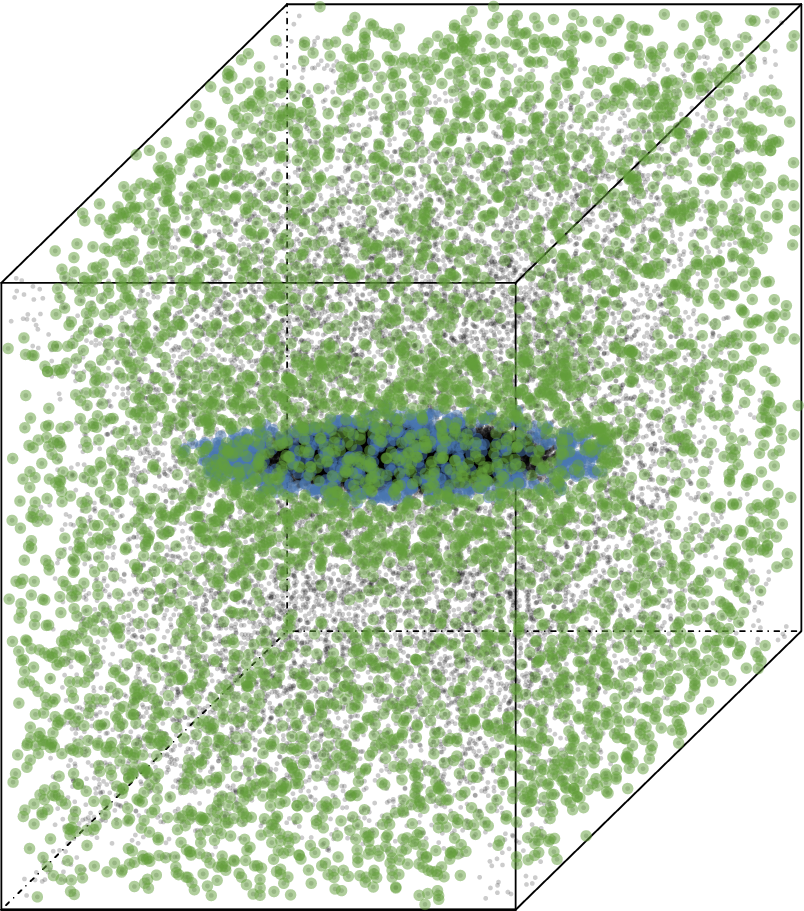
\includegraphics[keepaspectratio=true, width=\textwidth, height=0.23\textheight]{discussion/img/baakman_1_60000_anisotropy.png}
					\caption{\baakmanOne [\num{2.955638611296131e+00}, \num{4.876641609906340e+00}]}
					\label{fig:discussion:anisotropy:baakman1}
				\end{subfigure}	
				\subfigvspace
				\begin{subfigure}{0.23\textwidth}
					\centering
					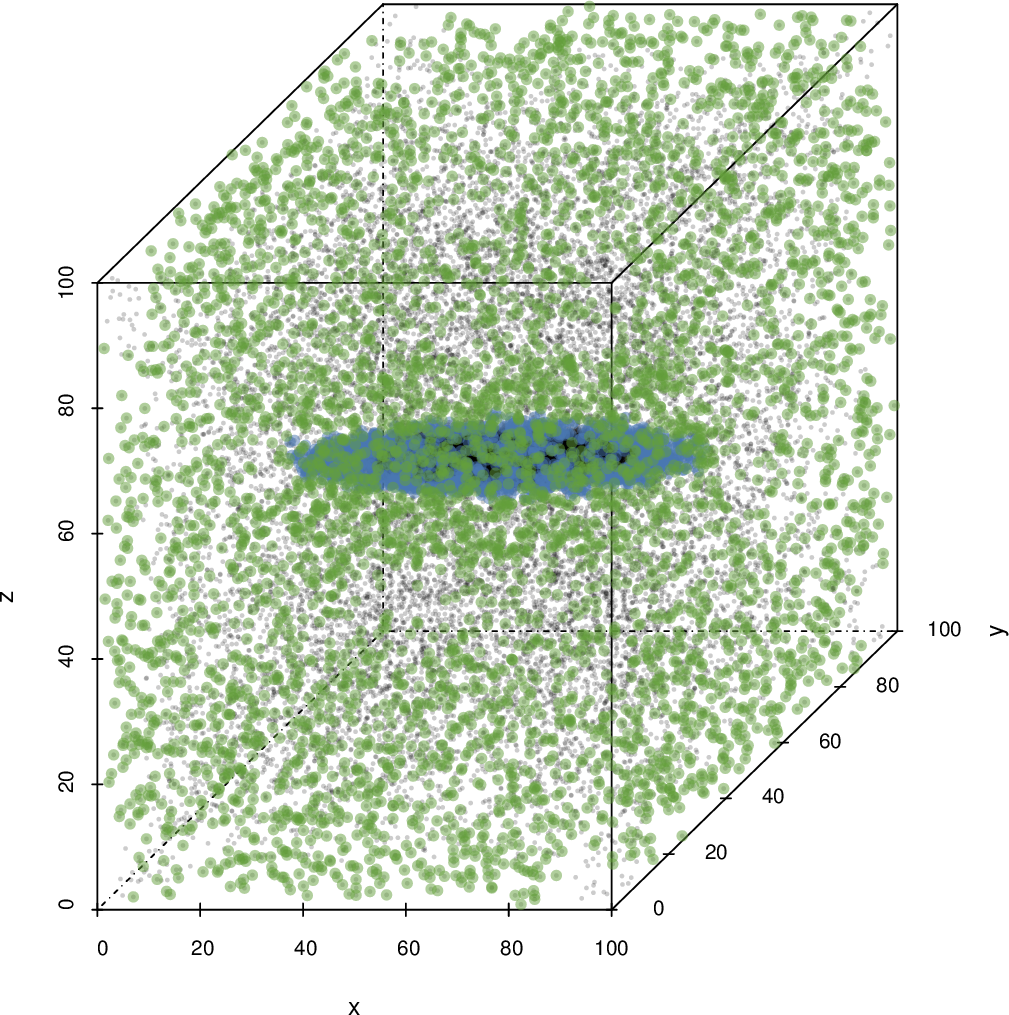
\includegraphics[keepaspectratio=true, width=\textwidth, height=0.23\textheight]{discussion/img/baakman_4_60000_anisotropy.png}
					\caption{\baakmanFour [\num{3.105833113039985e+00}, \num{5.987200775539245e+00}]}
					\label{fig:discussion:anisotropy:baakman4}
				\end{subfigure}		
				\begin{subfigure}{0.23\textwidth}
					\centering
					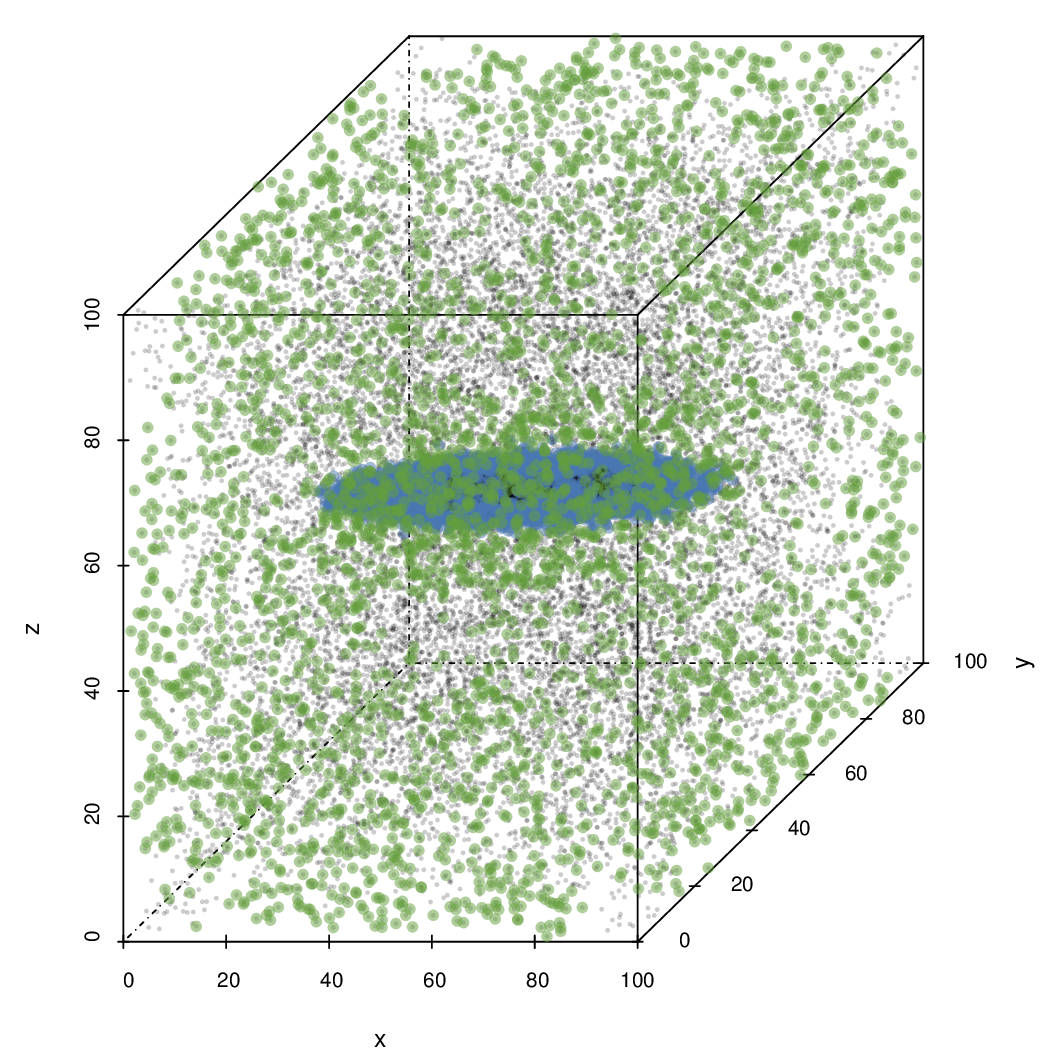
\includegraphics[keepaspectratio=true, width=\textwidth, height=0.23\textheight]{discussion/img/baakman_5_60000_anisotropy.png}
					\caption{\baakmanFive [\num{3.546238846198991e+00}, \num{8.192210308245695e+00}]}
					\label{fig:discussion:anisotropy:baakman5}
				\end{subfigure}			
				\caption{Scatter plots of data set
					\subref{fig:discussion:anisotropy:ferdosi1} \ferdosiOne, %
					\subref{fig:discussion:anisotropy:baakman1} \baakmanOne, %
					\subref{fig:discussion:anisotropy:baakman4} \baakmanFour, and %
					\subref{fig:discussion:anisotropy:baakman5} \baakmanFive. %
					The points with kernels whose anisotropy lies in the \nth{90} percentile are shown larger, and colored. The anisotropy range of the kernels of the emphasized points is shown below the plots.}
				\label{fig:discussion:anisotropy:singleSphere}
			\end{figure}
			%	
			\Cref{fig:discussion:anisotropy:singleSphere} shows the data sets with a single Gaussian with points whose anisotropy lie in the \nth{90} percentile emphasized. 
				% Ferdosi 1 & Baakman 1
				Hardly any differences are visible between the plots of data set \ferdosiOne and \baakmanOne. 
					% Very few points from Gaussian comonent
					In \cref{fig:discussion:anisotropy:ferdosi1,fig:discussion:anisotropy:baakman1} \percentage{5.180481283422460e-01} and \percentage{1.174799465240642e+01}, respectively, of the emphasized points are sampled from the Gaussian component of the data sets. This shows that the kernels in data set \baakmanOne are influenced by the increase in anisotropy compared to the isotropy of the Gaussian component in data set \ferdosiOne.
					% Shell of points sampled from the noise around the Gaussian comonent
					Furthermore a shell of points sampled from the noise with kernels whose anisotropy is relatively high surrounds the Gaussian component. It is quite likely that the shape of these kernels is influenced by the Gaussian component.
					% Explanation: high density -> anisotropy detection fails
					We expect that nearer to the mean of the Gaussian component fewer kernels are influenced by its anisotropy as the physical density of points is quite high in that area. Consequently the volume of the local neighborhood is quite low and thus possibly insufficient to represent the shape of the Gaussian.
				% Baakman 4 and 5
				In data set \baakmanFour and \baakmanFive a larger percentage of the points with a kernel whose anisotropy is relatively high is sampled from the Gaussian component, \percentage{2.190842245989305e+01} and \percentage{4.207887700534759e+01}, respectively. 
				% Conclusion
				Therefore we tentatively conclude that as the anisotropy of the Gaussian component increases, the anisotropy of the kernels of the points near that component increases as well.
		
	% Multi Sphere
		\begin{figure}
			\centering
			\begin{subfigure}{0.23\textwidth}
				\centering
				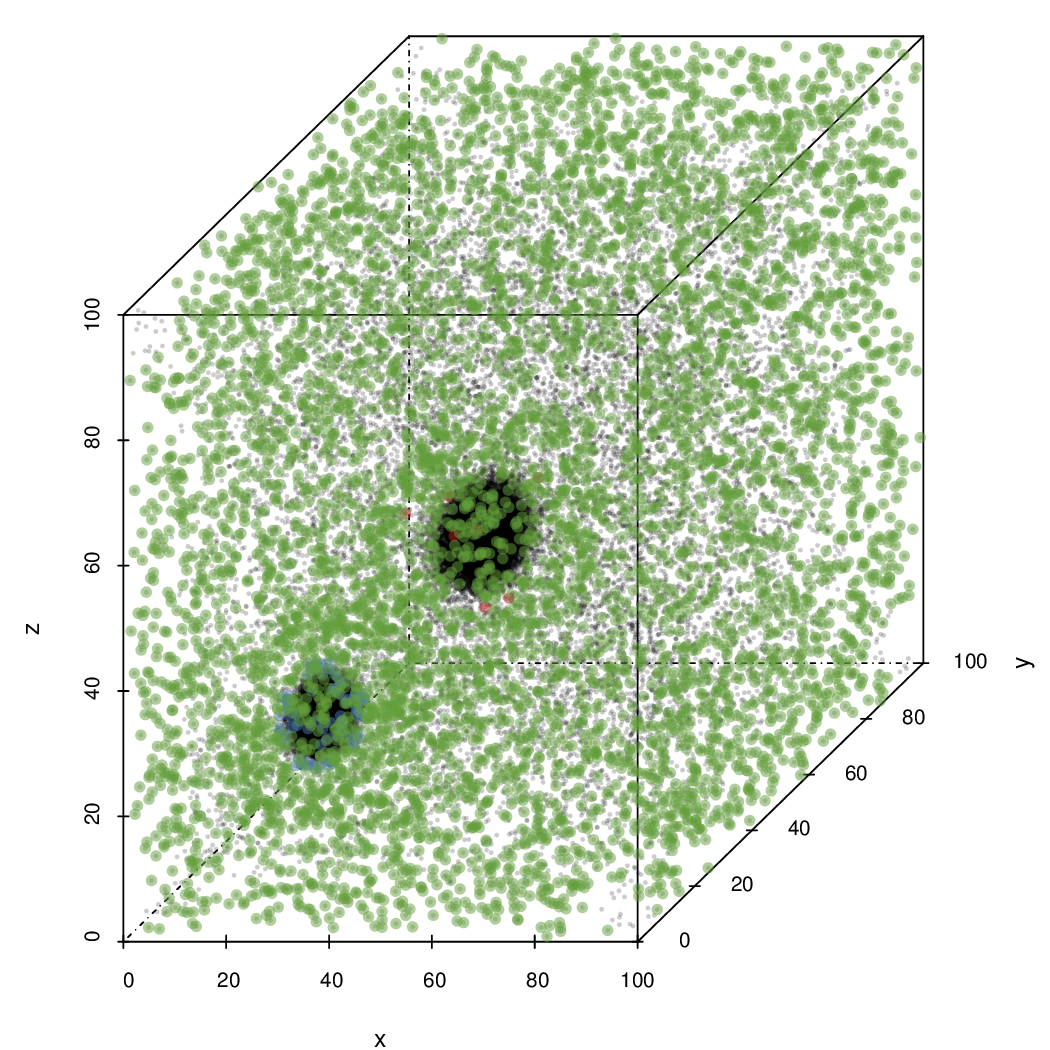
\includegraphics[keepaspectratio=true, width=\textwidth, height=0.23\textheight]{discussion/img/ferdosi_2_60000_anisotropy.png}
				\caption{\ferdosiTwo [\num{2.215970619635167e+00}, \num{5.678002691654005e+00}]}
				\label{fig:discussion:anisotropy:ferdosi2}
			\end{subfigure}
			\begin{subfigure}{0.23\textwidth}
				\centering
				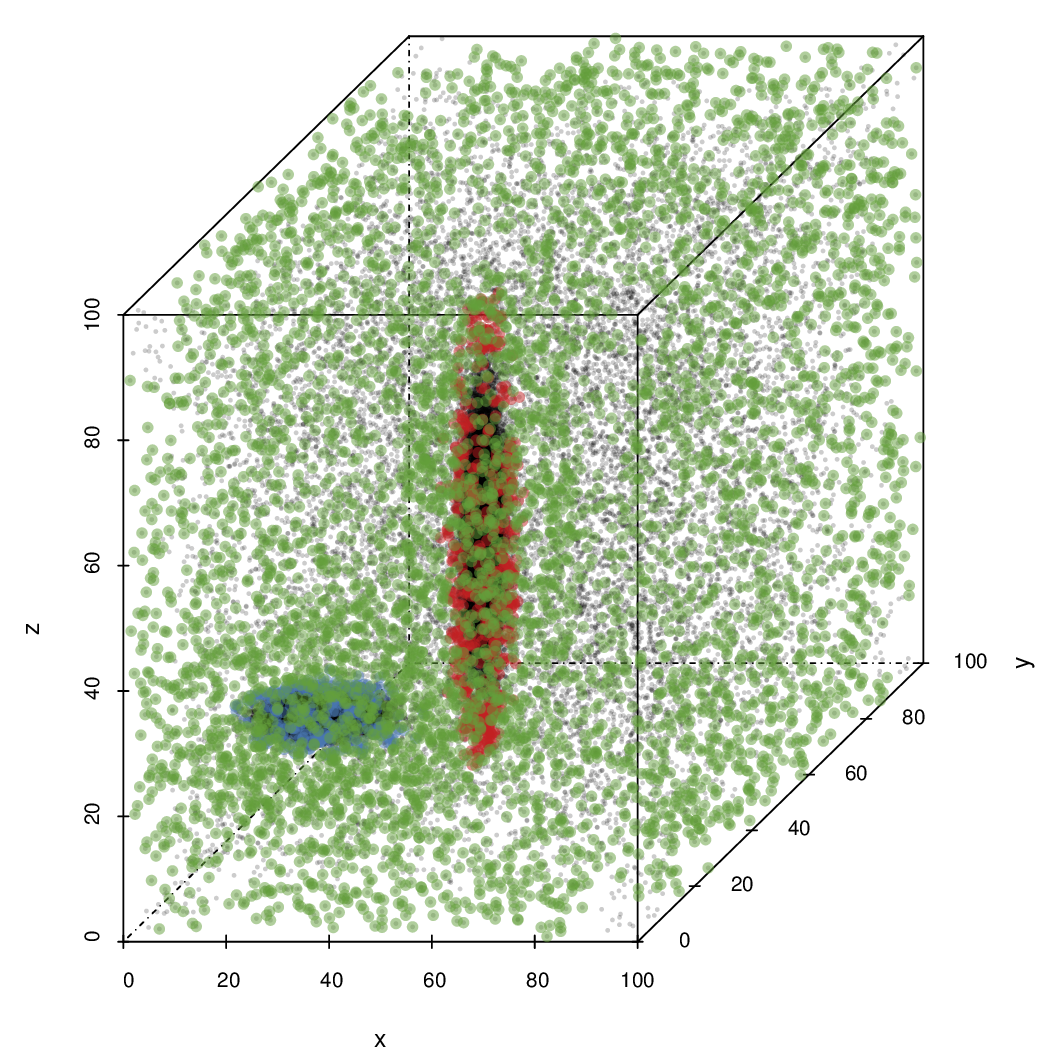
\includegraphics[keepaspectratio=true, width=\textwidth, height=0.23\textheight]{discussion/img/baakman_2_60000_anisotropy.png}
				\caption{\baakmanTwo [\num{2.463414286522871e+00}, \num{7.134567710248723e+00}]}
				\label{fig:discussion:anisotropy:baakman2}
			\end{subfigure}	
			\subfigvspace
			\begin{subfigure}{0.23\textwidth}
				\centering
				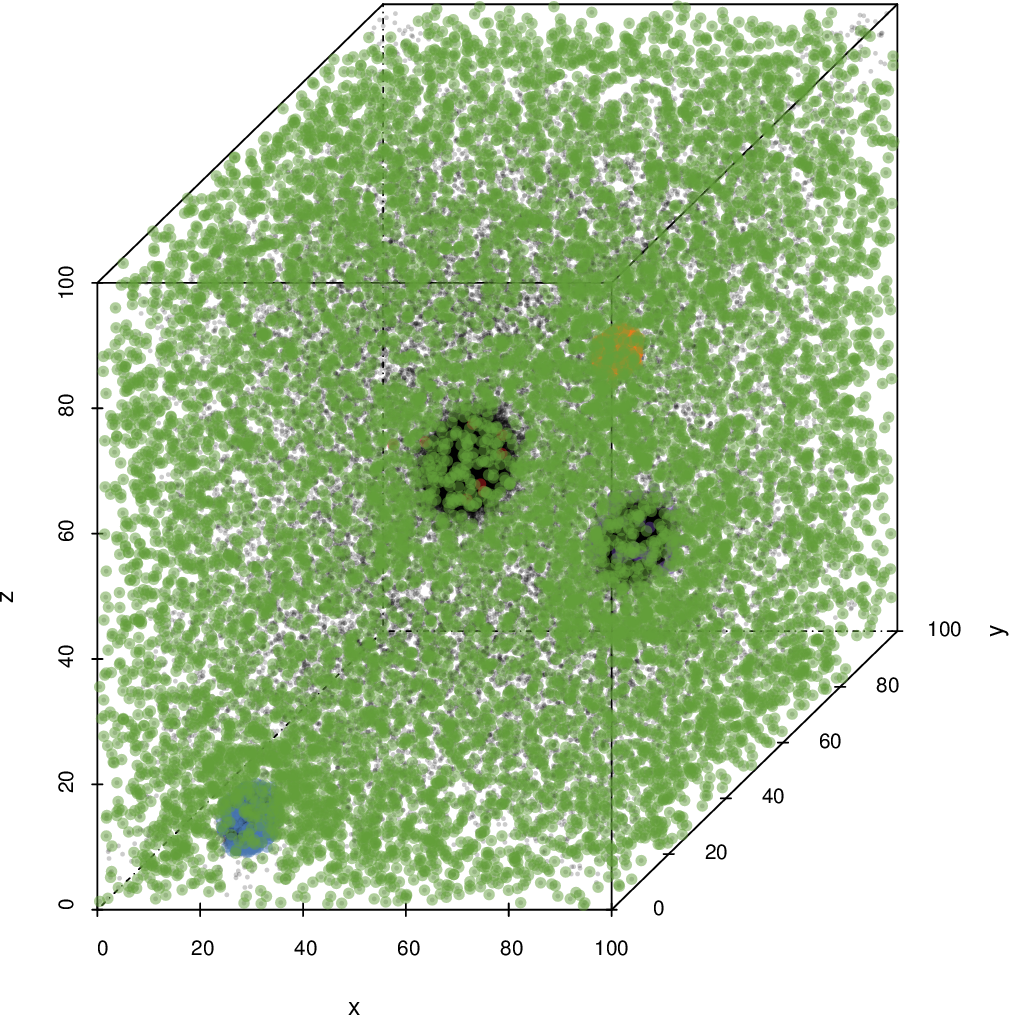
\includegraphics[keepaspectratio=true, width=\textwidth, height=0.23\textheight]{discussion/img/ferdosi_3_120000_anisotropy.png}
				\caption{\ferdosiThree [\num{2.138909227329211e+00}, \num{8.855946762727447e+00}]}
				\label{fig:discussion:anisotropy:ferdosi3}
			\end{subfigure}		
			\begin{subfigure}{0.23\textwidth}
				\centering
				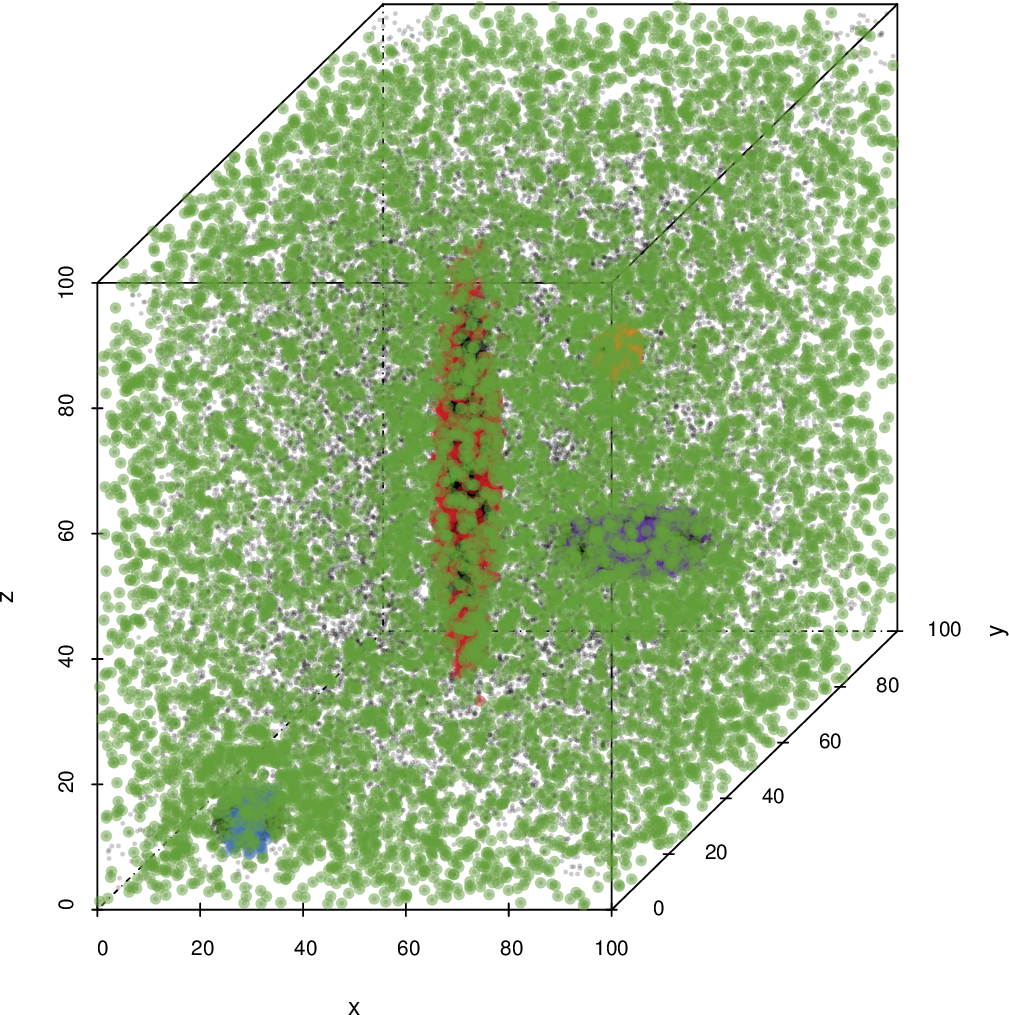
\includegraphics[keepaspectratio=true, width=\textwidth, height=0.23\textheight]{discussion/img/baakman_3_60000_anisotropy.png}
				\caption{\baakmanThree [\num{2.316497642958064e+00}, \num{8.855946762727445e+00}]}
				\label{fig:discussion:anisotropy:baakman3}
			\end{subfigure}			
			\caption{Scatter plots of set
				\subref{fig:discussion:anisotropy:ferdosi2} \ferdosiTwo, %
				\subref{fig:discussion:anisotropy:baakman2} \baakmanTwo, %
				\subref{fig:discussion:anisotropy:ferdosi3} \ferdosiThree, and %
				\subref{fig:discussion:anisotropy:baakman3} \baakmanThree. %
				The points that have an anisotropy in the \nth{90} percentile are shown larger and colored. Below each plot the range of the anisotropy of the kernels of the emphasized points is shown.}
			\label{fig:discussion:anisotropy:multisphere}
		\end{figure}			
		% General Introduction
		\Cref{fig:discussion:anisotropy:multisphere} emphasizes the points with the most anisotropic kernels in data set \ferdosiTwo through \baakmanThree. 
		% Ferdosi 2
			% Same observations as for ferdosi 1, present percentages
			In the plot associated with data set \ferdosiTwo we observe the same shells of points with highly anisotropic kernels around the Gaussian components as in data set \ferdosiOne. Another similarity between these two data sets is that very few points sampled from the Gaussian component have a kernel with high anisotropy; \percentage{1.453877} and \percentage{0.1169786} of the points with a high anisotropy are sampled from the first and second Gaussian component, respectively. 
			% F2G1 vs F2G2
			We contribute the difference in the number of highly anisotropic kernels associated with data points sampled from the two Gaussian components to the difference in the volume of the their eigenspheres.
		% Baakman 2
			% More points near the Gaussian anisotropic
			For \cref{fig:discussion:anisotropy:baakman2} we find that the increase in anisotropy of the components causes \percentage{4.328209} and \percentage{8.656417} of the kernels with high anisotropy to be associated with a point sampled from `Trivariate Gaussian 1' and 2, respectively. 
		% Ferdosi 3
			% G1 and G3 have anisotropic kernels. 
			Interestingly in data set \ferdosiThree, two of the four spherical Gaussians, `Trivariate Gaussian 1' and 3, are associated with respectively \percentage{1.404095} and \percentage{2.223151} of the highly anisotropic kernels. Whereas no point sampled from `Trivariate Gaussian 2' or 4 has a kernel with high anisotropy.
			% Relate to results: components with highest sd, lowest means, lower density -> larger variation in anisotropy
			Comparing the mean kernel anisotropy in \cref{tab:results:multiSphere:anisotropy} we find that relative to the other Gaussian components in \ferdosiThree, `Trivariate Gaussian 1' and 3 have a relatively low mean anisotropy. However their standard deviations are relatively high, suggesting that in these components some kernels are extremely anisotropic, whereas others are near isotropic. We contribute this difference within the points sampled from these Gaussian components to differences in the physical densities of the neighborhoods around the means, as we did for data set \ferdosiOne and \baakmanOne.
			% Why G1 and G3 and not G2 and G4? 
			Component one and four of data set \ferdosiThree differ from the other Gaussian components in two aspects: firstly the volume of their eigenspheres is relatively low and secondly they are placed near the boundaries of the data set. 
				% G1/G3 are placed near the  border of the data set, contrast with results of F3Noise?
				\Cref{fig:discussion:ferdosi3Noise:anisotropy} shows that the distance to the limits of the background does not explain the difference in anisotropy of the kernel, as in that figure the first and third component of \ferdosiThreeNoise have more anisotropic kernels than the other components, even though they are farther away from the boundary of the data set.
				% G1/G3 have lower covariance:
				The first explanation fits with the observations from \cref{s:results} that components with eigenspheres with larger volumes, have kernels that have a higher anisotropy.
		% Baakman 3
			In data set \baakmanThree we observe the same effect as in \ferdosiThree but stronger; from the points with the most anisotropic kernels more are sampled from the two densest Gaussian component than from the other components. 

	% Some general conclusion
	\Cref{fig:discussion:anisotropy:singleSphere,fig:discussion:anisotropy:multisphere} show that the overwhelming majority of the points with a relative highly anisotropic kernel are sampled from the `Uniform random background'. We contribute this to the covariance matrix being sensitive to fine, random structures in the noise, that give the impression of anisotropy in the data where there is none.

% Denser component -> higher anisotropy of kernels
	In \cref{s:results} we observed that both the volume of the eigensphere and the anisotropy of the Gaussian component influenced the anisotropy of the kernels. To test which factor is responsible for the difference in anisotropy we introduce two new data sets: \anisotropyOne and \anisotropyTwo.
	% Definition
	To create data set \anisotropyOne the covariance matrix used in \ferdosiOne was replaced by $\diag([4, 3, 1])$, data set \anisotropyTwo is the same as \anisotropyOne but uses $3 \cdot \diag([4, 3, 1])$.
	% Same anisotropy, different eigensphere volume
	Consequently the Gaussian components of \anisotropyOne and \anisotropyTwo have the same anisotropy, but the volumes of the eigenspheres of their covariance matrices differ.
	% Influence of density on MSE
	%
	\begin{table}
		\centering
		%!TEX root = ../../paper.tex

\begin{tabular}{l*{2}{S[scientific-notation=true, round-mode=places,round-precision=3]}}
\toprule
~ 				& \multicolumn{2}{c}{Estimator}\\ \cmidrule{2-3}
Set				& {\mbe}					& {\sambe}	\\
\midrule
\ferdosiOne		& 8.30580618349064E-09		&  8.9087329457441E-09 \\
\baakmanOne		& 1.49022877061299E-08		&  1.5398737157543E-08 \\	
\baakmanFour	& 2.93709420107411E-08		&  2.9634323205557E-08 \\	
\baakmanFive	& 5.57179476550916E-08		&  5.5847473903432E-08 \\	
\bottomrule
\end{tabular}
		\caption{Performance of the Modified Breiman Estimator with fixed-shaped and shape-adaptive kernels on the data sets \anisotropyOne and \anisotropyTwo.} 	
		\label{tab:discussion:anisotropy:mse}
	\end{table}
	%
	The \mses of the two estimators on data set \anisotropyOne and \anisotropyTwo are shown in \cref{tab:discussion:anisotropy:mse}. Clearly both estimators perform better on the data set with higher values on the diagonal of the covariance matrix of the Gaussian component.
	% Influence of density on Anisotropy
	\Cref{fig:discussion:anisotropy:anisotropy} illustrates the influence of the volume of the eigensphere of the Gaussian component on the anisotropy of the kernels near that component. Of the points with a highly anisotropic kernel in data set \anisotropyOne \percentage{6.233289} is sampled from the Gaussian component, in data set \anisotropyTwo this is \percentage{4.161096}. Although the difference is small, it illustrates that the volume of the eigensphere of a component influences the anisotropy of the kernels. 
	% THE PLOT
	\begin{figure}
		\centering
		\begin{subfigure}{0.23\textwidth}
			\centering
			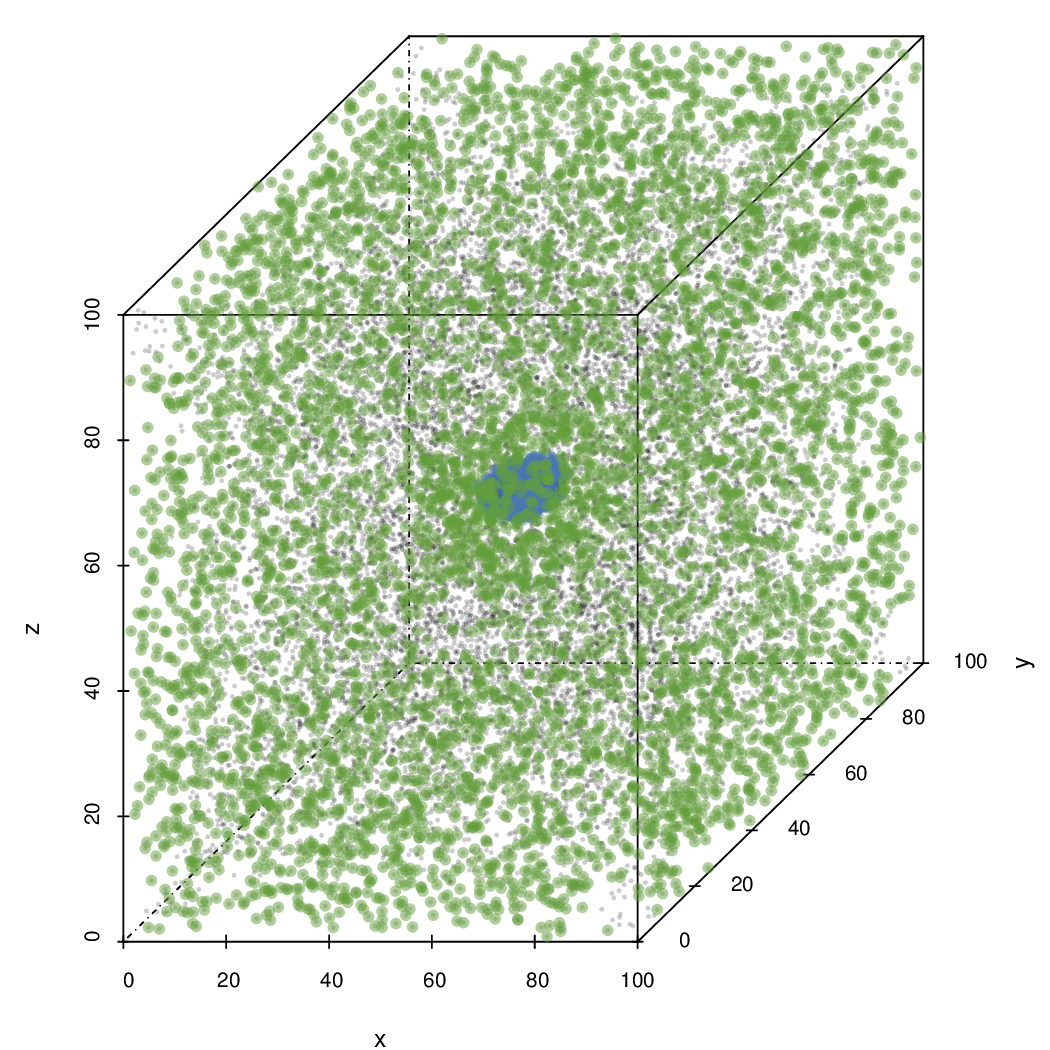
\includegraphics[keepaspectratio=true, width=\textwidth, height=0.23\textheight]{discussion/img/anisotropy_1_60000_anisotropy.png}
			\caption{\anisotropyOne}
			\label{fig:discussion:anisotropy:anisotropy1}
		\end{subfigure}
		\begin{subfigure}{0.23\textwidth}
			\centering
			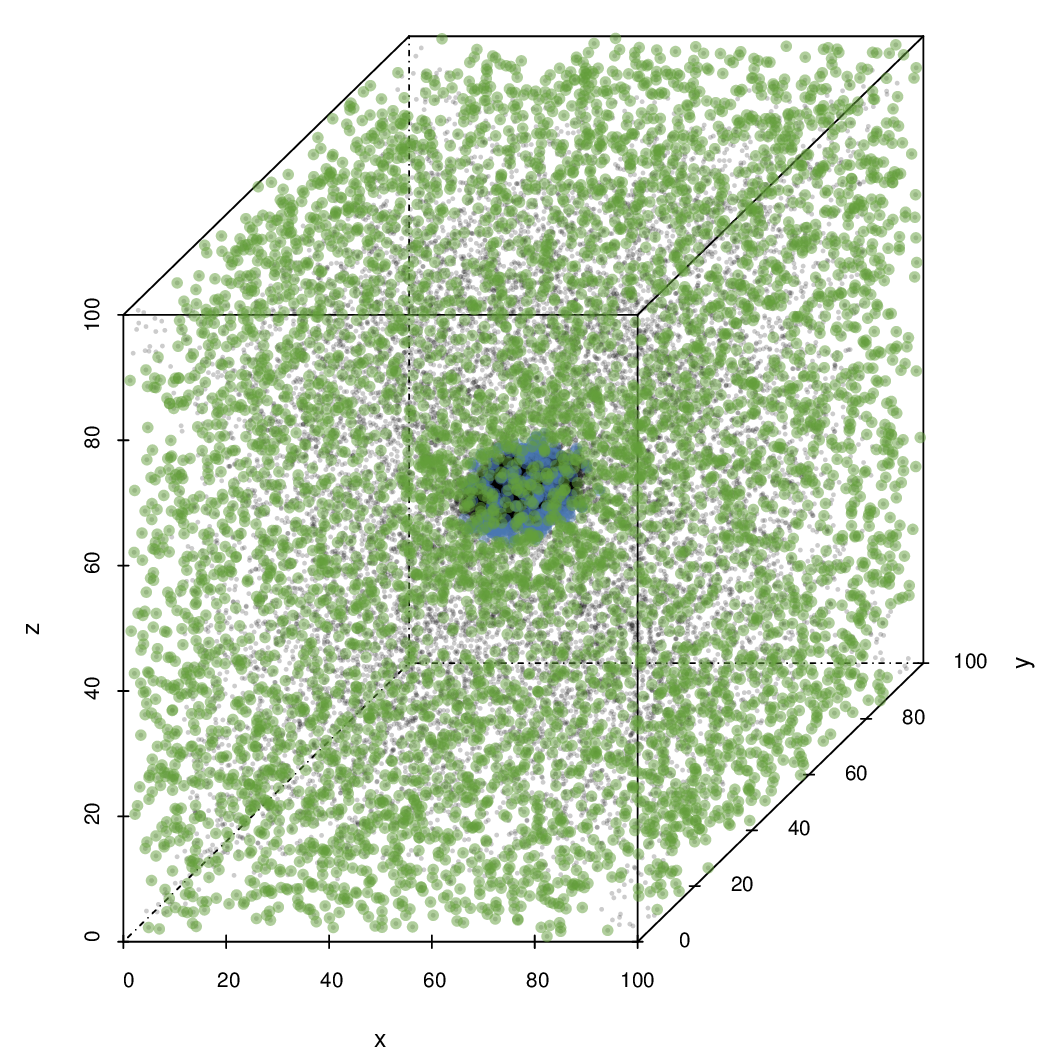
\includegraphics[keepaspectratio=true, width=\textwidth, height=0.23\textheight]{discussion/img/anisotropy_2_60000_anisotropy.png}
			\caption{\anisotropyTwo}
			\label{fig:discussion:anisotropy:anisotropy2}
		\end{subfigure}	
		\caption{Scatter plot of data set \subref{fig:discussion:anisotropy:anisotropy1} \anisotropyOne and \subref{fig:discussion:anisotropy:anisotropy2} \anisotropyTwo, with emphasized the points whose kernels have an anisotropy in the \nth{90} percentile.}
		\label{fig:discussion:anisotropy:anisotropy}
	\end{figure}

% Some conclusion